% Chapter 1. Introduction.
% Every number in this chapter comes from verify/registry.json, from
% figures/literature_values.json, or from the paper cited next to it.

\chapter{Introduction}
\label{ch:intro}

This report describes Phase 1 of an M.Tech.\ project on the atmosphere of Venus. It
starts from the first reading of the literature and ends with the proposal for Phase 2.
The subject is a single long-standing problem: something in the clouds of Venus absorbs
near-ultraviolet sunlight, and nobody knows what it is. This chapter explains what is
known about that problem, what has been tried, and how this project approaches it
differently.

\section{Venus and its clouds}
\label{sec:venus}

Venus has a thick atmosphere. The pressure at the surface reaches 92 bar and the surface
temperature is about 750~K~\cite{dai2025review}. The planet is completely covered by a
dense cloud deck that lies between 47 and about 70~km above the surface and is more than
20~km thick~\cite{dai2025review}. The clouds are made of small droplets of concentrated
sulfuric acid, H\sub{2}SO\sub{4}~\cite{dai2025review}.

Measurements made by a descent probe divide the cloud deck into three layers by the mass
of cloud material they hold: the lower cloud, from about 48 to 50~km; the middle cloud,
from about 50 to 56~km; and the upper cloud, from about 56 to 70~km~\cite{dai2025review}.
The droplets are also grouped by size into \emph{modes}. Mode~1 droplets are smaller than
one micrometre across and are the most numerous throughout the cloud deck; mode~2
droplets are about two micrometres across~\cite{dai2025review}. Mode~1 matters for this
report because the unknown absorber is now thought to be mixed into mode~1
droplets~\cite{dai2025review,perezhoyos2018}.

The \emph{cloud top} is defined as the height at which the optical depth of the cloud,
counted downward from space, reaches one~\cite{dai2025review}. Optical depth is a
measure of how much light a layer removes: light that crosses an optical depth of one
keeps a fraction $e^{-1}$, about a third, of its original intensity. Depending on the
wavelength used and the place observed, the cloud top lies between 65 and
72~km~\cite{dai2025review}.

The solid planet turns very slowly. One rotation relative to the stars takes 243 Earth
days, and one solar day, from noon to noon, takes 117 Earth days~\cite{bertaux2016}. The
atmosphere at the cloud top moves far faster. It travels westward round the planet in
about four days, with a wind speed of about 100 metres per
second~\cite{bertaux2016}; in the cloud layer as a whole the circuit takes 4 to 6
days~\cite{limaye2018}. This fast circulation is called \emph{super-rotation}. It was
first revealed by ultraviolet observations of the cloud markings (Ross, 1928, and Boyer
and Camichel, 1961, as cited in~\cite{perezhoyos2018}), which is the first sign that the
ultraviolet appearance of Venus and its atmospheric motion are linked.

Figure~\ref{fig:F1} summarises this structure. It also shows two things that come from
the present project and are explained later: the grey band, which marks the altitudes
where the model's radiation responds to the absorber (Chapter~5), and the altitudes where
the model's own chemistry places a set of candidate molecules (Chapter~6).

\begin{figure}[htbp]
  \centering
  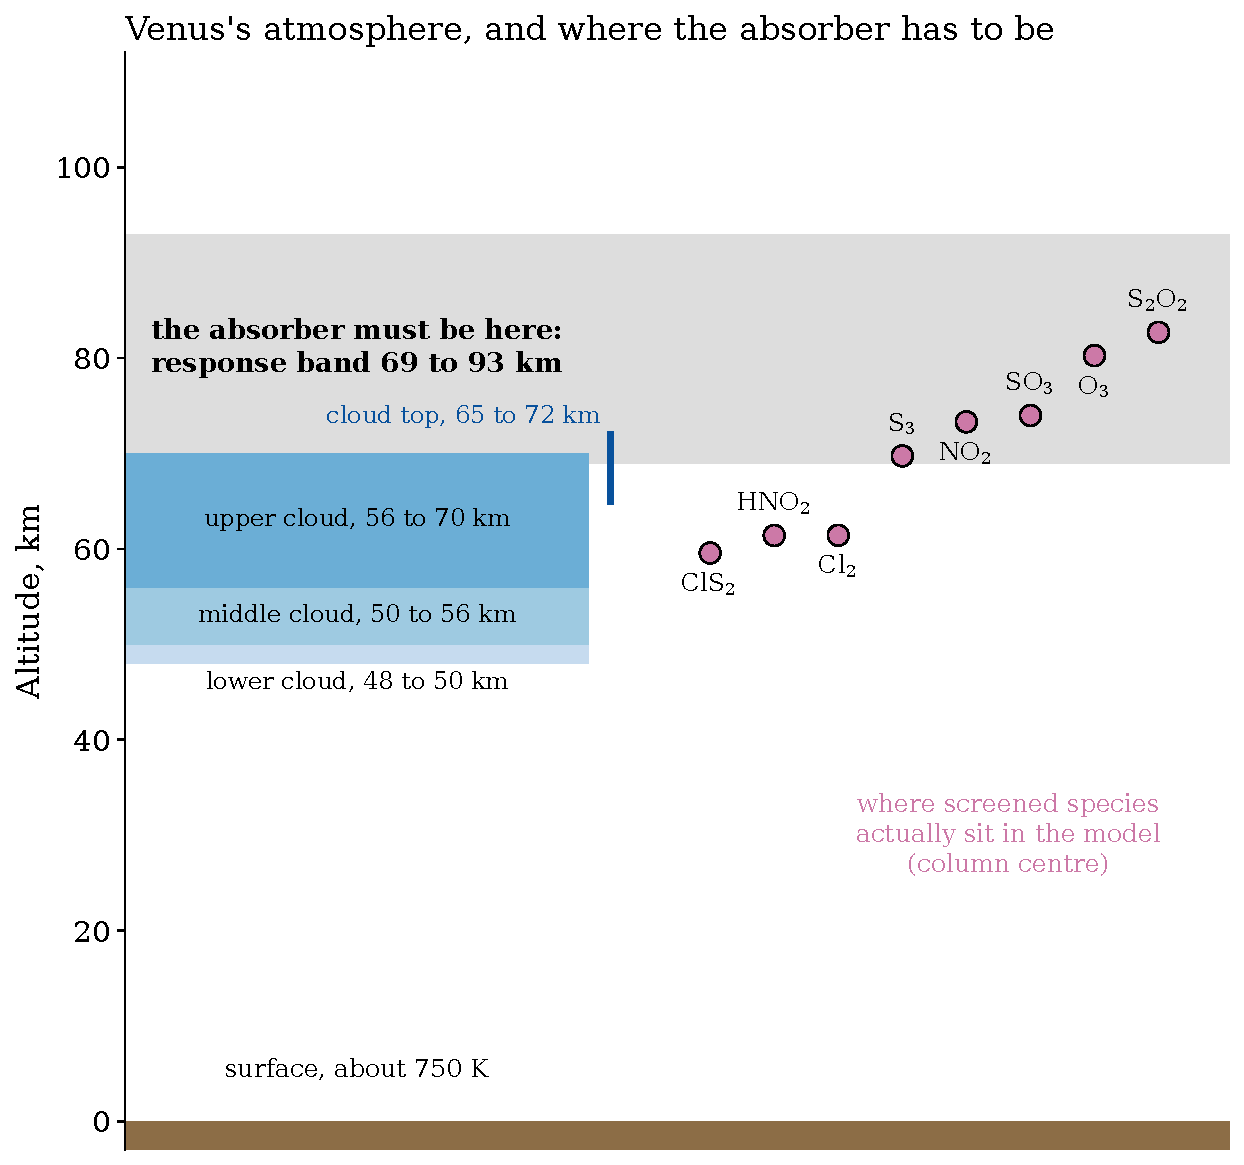
\includegraphics[width=0.68\textwidth]{F01_CTX_venus-atmosphere_ch1_s3.pdf}
  \caption[The Venus atmosphere, and where the absorber has to be]{The Venus atmosphere, and where the absorber has to be. Left: the three cloud
    layers and the range of cloud top heights, from~\cite{dai2025review}; the surface
    temperature, from the same source. Grey band: the response band, 69 to 93~km,
    found in Experiment~6 (Chapter~5). Purple circles: the column centre of eight
    candidate molecules as placed by the model's own chemistry (Experiment~12).
    Sources: \texttt{figures/literature\_values.json}; registry keys
    \texttt{e6.interval.90.lo}, \texttt{e6.interval.90.hi} and
    \texttt{e12.<species>.centroid}.}
  \label{fig:F1}
\end{figure}

\section{The unknown ultraviolet absorber}
\label{sec:absorber}

In visible light Venus is very bright: its clouds scatter about 80 per cent of the
incoming sunlight back to space~\cite{dai2025review}. Towards the ultraviolet the planet
becomes darker, and the darkening has two parts. Below 320~nm the shape of the absorption
matches sulfur dioxide, SO\sub{2}, which is therefore taken to be responsible for
it~\cite{dai2025review}. But SO\sub{2} absorbs only weakly at longer wavelengths, and its
effect is negligible beyond 320~nm~\cite{perezhoyos2018}. Between 320 and 400~nm there is
a second, strong absorption that no known species has been shown to
explain~\cite{dai2025review}. In the spectrum of the planet it appears as a broad band
reaching from the near ultraviolet into the blue~\cite{perezhoyos2018}. Because its
carrier is not known, it is called the \emph{unknown ultraviolet
absorber}~\cite{dai2025review}. In this report it is called simply \emph{the absorber}.

Figure~\ref{fig:F2} shows the problem directly. The upper panel is one reflectivity
spectrum of Venus, number 151, measured by the MESSENGER spacecraft during its second
Venus flyby on 5 June 2007~\cite{perezhoyos2018}. Reflectivity, written $I/F$, is the observed radiance divided
by $\pi F_\odot$, where $F_\odot$ is the solar flux arriving at Venus~\cite{perezhoyos2018}:
a perfectly white, evenly scattering surface lit from directly overhead would have
$I/F = 1$. The lower panel is the
absorption cross section of SO\sub{2} used in the model, which measures how strongly one
SO\sub{2} molecule absorbs at each wavelength. Venus is dark between 320 and 400~nm, which
is exactly where SO\sub{2} has almost stopped absorbing. From the same MESSENGER data,
P\'erez-Hoyos et al.\ found the absorption to be centred near 340~nm with a full width at
half maximum of about 140~nm~\cite{perezhoyos2018}.

\begin{figure}[htbp]
  \centering
  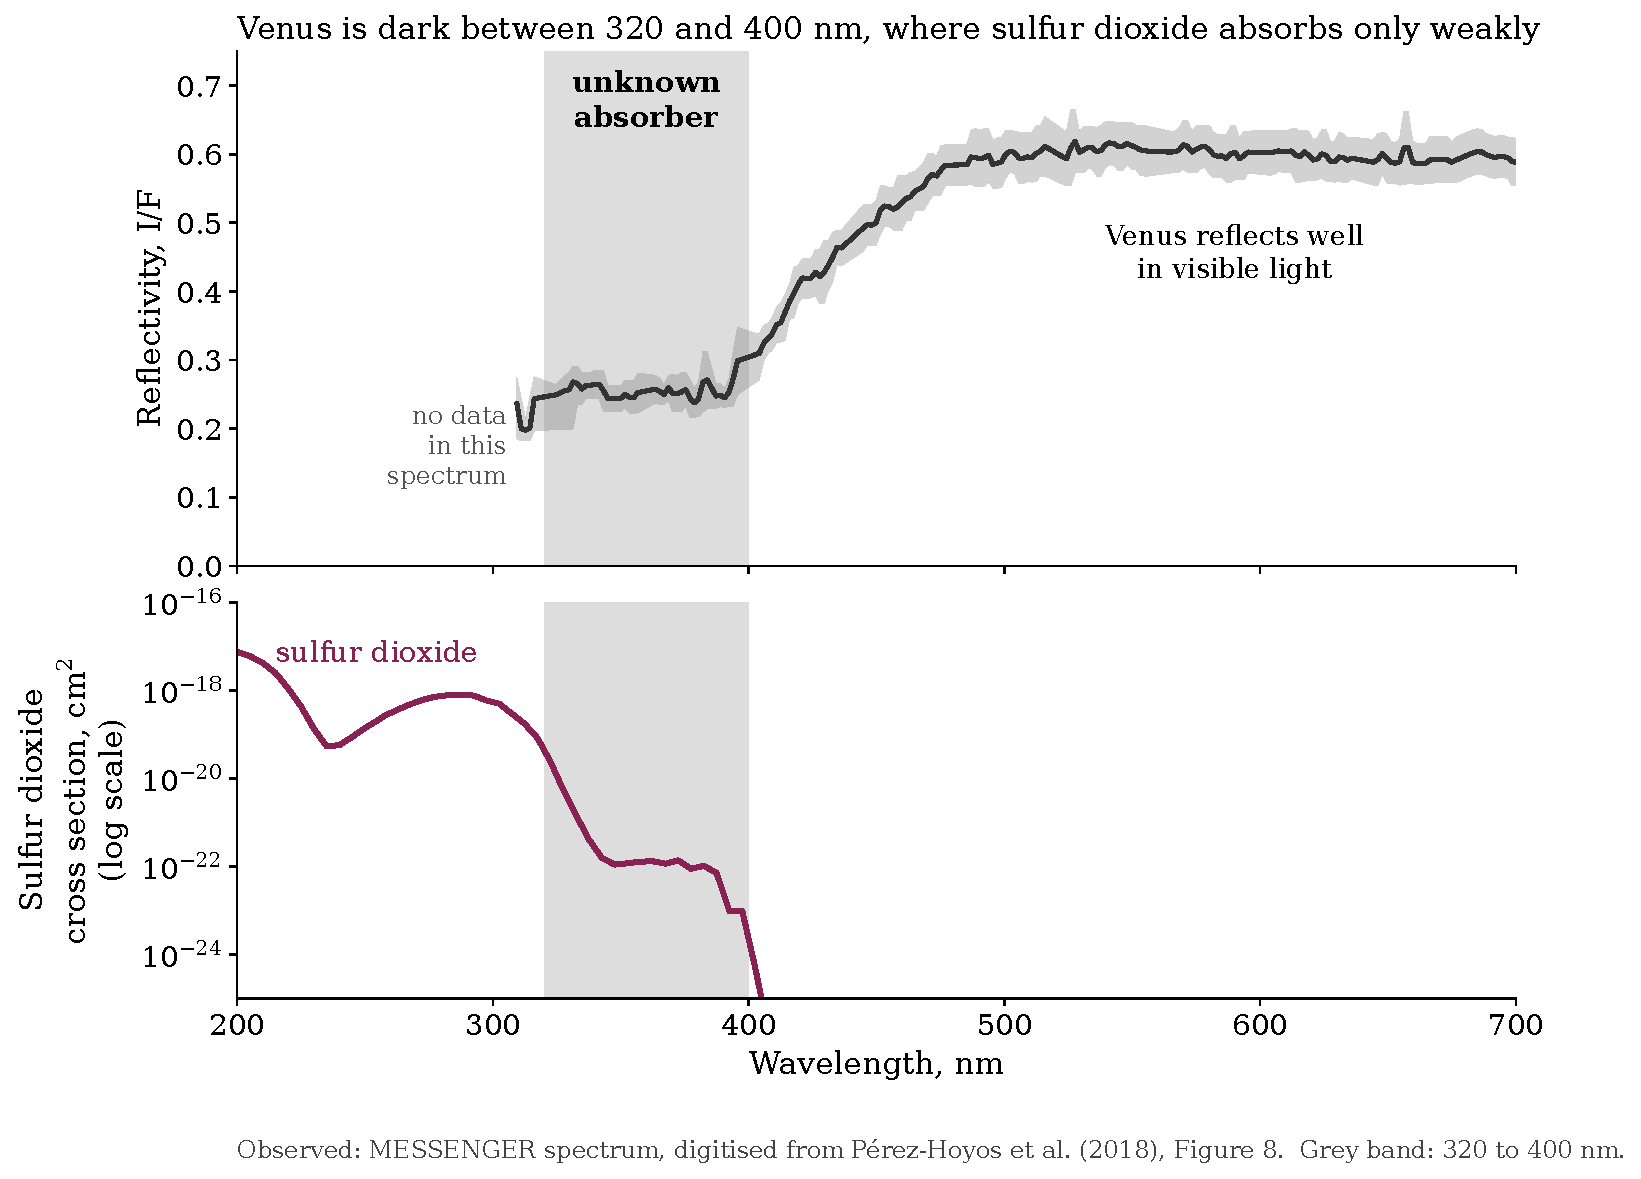
\includegraphics[width=0.74\textwidth]{F02_CTX_observed-uv-absorption_ch1_s2.pdf}
  \caption[Venus is dark between 320 and 400~nm, where sulfur dioxide absorbs only weakly]{Venus is dark between 320 and 400~nm, where sulfur dioxide absorbs only
    weakly. Top: observed reflectivity $I/F$ of MESSENGER spectrum 151, digitised from
    Figure~8 of P\'erez-Hoyos et al.~\cite{perezhoyos2018}; the shaded envelope is the
    drawn observation with its plotted error range, and the line its middle. Bottom: the SO\sub{2} absorption cross section used in
    the model, on a logarithmic scale. Sources:
    \texttt{figures/data/perez-hoyos-2018-fig8-IF.csv} (with its provenance file) and
    \texttt{thermo/photo\_cross/SO2/SO2\_cross.csv}.}
  \label{fig:F2}
\end{figure}

The absorber matters for three reasons.

\textbf{It heats the cloud top.} Observations and models agree that the absorber is
responsible for about half of the solar heating at the cloud top~\cite{dai2025review}.
Solar heating in the upper clouds has in turn been proposed as one of the engines of the
super-rotation, through the thermal tides it excites~\cite{perezhoyos2018}.

\textbf{It changes over time, and the circulation changes with it.} The brightness of
Venus at 365~nm varied strongly between 2006 and 2017, which implies that the amount of
absorber varied by a factor of two; the resulting change in solar heating has been
proposed to alter the strength of the Hadley circulation, the large overturning flow
between the equator and the poles (Lee et al.,
2019, as reviewed in~\cite{dai2025review}).

\textbf{Its pattern traces vertical motion.} The dark and bright markings seen in
ultraviolet images are not random. At low latitudes the clouds are dark because
convection brings the absorber up from below; at middle latitudes a cold layer with a
stable temperature profile suppresses vertical mixing and cuts off that supply, so the
clouds there are bright and uniform~\cite{titov2008}. In other words, where the absorber
appears depends on how the atmosphere moves it up and down. This observation is the
starting point of the present project.

What is known about \emph{where} the absorber sits is limited. Measurements of sunlight
made by descent probes found that ultraviolet absorption happens mainly in the upper
cloud, above about 57~km, and is negligible in the middle and lower clouds (Tomasko et
al., 1980, and Ekonomov et al., 1984, as reviewed in~\cite{dai2025review}). The supply of
absorber from below appears to be continuous at low latitudes~\cite{dai2025review}.
Nearly a century after the ultraviolet contrasts were first photographed from Earth, the
substance that causes them is still unknown~\cite{limaye2018}.

\section{The candidates proposed so far}
\label{sec:candidates}

Many substances have been put forward as the absorber. Table~\ref{tab:candidates} lists
the main ones, as summarised in a recent review~\cite{dai2025review} and in the
MESSENGER study~\cite{perezhoyos2018}. The table is a summary for orientation; Chapter~2
reviews the key papers one by one.

\begin{table}[htbp]
  \centering
  \caption[The main candidates for the unknown absorber, what supports each, and what counts against it]{The main candidates for the unknown absorber, what supports each, and what
    counts against it. Proposers are given as cited in the sources in the last column.}
  \label{tab:candidates}
  \footnotesize
  \setstretch{1.0}
  \begin{tabularx}{\textwidth}{>{\raggedright\arraybackslash}p{2.6cm}
                                >{\raggedright\arraybackslash}X
                                >{\raggedright\arraybackslash}X
                                >{\raggedright\arraybackslash}p{1.3cm}}
    \toprule
    Candidate & In its favour & Against it & Source \\
    \midrule
    Sulfur dioxide, SO\sub{2} &
      Matches the absorption below 320~nm. &
      Negligible beyond 320~nm, so it cannot supply the band between 320 and 400~nm. &
      \cite{perezhoyos2018,dai2025review} \\
    Polysulfur, S\sub{x} (Hapke and Nelson, 1975) &
      One of the first candidates considered for its spectral properties. &
      No single form matches the observed spectrum; it does not dissolve in sulfuric
      acid and would spoil an optical effect, the glory, that the droplets show. &
      \cite{dai2025review} \\
    Ferric chloride, FeCl\sub{3}, dissolved in the droplets (Zasova et al., 1981) &
      Spectral behaviour close to the absorber; dissolves in sulfuric acid. &
      Its absorption band is too narrow and too weak between 400 and 500~nm. &
      \cite{dai2025review} \\
    Disulfur monoxide, S\sub{2}O (Lo et al., 2003) &
      Good match between 400 and 500~nm. &
      Its absorption weakens quickly between 320 and 340~nm, where the absorber is still
      strong. &
      \cite{dai2025review} \\
    Disulfur dioxide, OSSO or S\sub{2}O\sub{2} &
      Its two forms, cis and trans, in comparable amounts, together match the spectrum
      between 330 and 420~nm, a result of Frandsen et al.\ reviewed
      in~\cite{dai2025review}. &
      A model of the clouds gives a mixing ratio at the cloud top of no more than one
      part in $10^{14}$, far too little~\cite{dai2024,dai2025review}; an independent
      study also finds it falls short~\cite{egan2025osso}. &
      \cite{dai2025review} \\
    Iron and sulfur minerals: rhomboclase and acid ferric sulfate &
      A mixture absorbs between 300 and 500~nm, consistent with the
      observations~\cite{jiang2024}. &
      Made under particular laboratory conditions; whether they exist in the clouds,
      and how much, is unknown. &
      \cite{dai2025review} \\
    Chlorine and sulfur compounds, such as SCl\sub{2} &
      Shown in the review among the candidates whose spectra come close to the
      absorber's. &
      The review gives no abundance for them in the clouds. &
      \cite{dai2025review} \\
    Organic ``red oil'' (Spacek and Benner, 2021) &
      A large organic molecule that dissolves in acid. &
      Listed in the review as a speculative hypothesis. &
      \cite{dai2025review} \\
    A mixture of several absorbers &
      Would explain the width of the band and its lack of fine structure. &
      Listed in the review as a possibility; not yet tested. &
      \cite{dai2025review} \\
    \bottomrule
  \end{tabularx}
\end{table}

Most of these proposals share one form of argument. A substance is measured in the
laboratory, or its spectrum is calculated, and the spectrum is compared with the observed
absorption. If the two look alike, the substance is put forward as a candidate. This
argument establishes one thing: that the substance absorbs at the right wavelengths. It
does not establish that enough of the substance can exist on Venus, and it does not
establish that the substance sits at the altitude where the absorption happens.

Those two further questions have been asked for a few candidates, one at a time. For
OSSO, a photochemical model showed that it is destroyed almost as soon as it forms, so its
abundance at the cloud top is far too small~\cite{dai2024,dai2025review}, and an
independent study reached the same conclusion~\cite{egan2025osso}. For polysulfur, model
calculations placed a large amount of it below the cloud base, and the same author later
concluded that it cannot explain the absorption in the upper clouds~\cite{dai2025review}.
The review itself concludes that a successful candidate must explain the observed
spectrum, must have the right distribution of abundance in the cloud layer, and must have
a stable source that keeps its abundance from being removed by chemistry and
mixing~\cite{dai2025review}. What was missing at the start of this project was a way to
ask these questions together, for every candidate, inside one model.

\section{The question this project asks}
\label{sec:question}

The question of this project is therefore not \emph{which molecule has the right
spectrum}. It is this: \textbf{can any proposed carrier be present in the right amount, at
the right altitude, and with the right spectral shape, all at once, inside a model that
is free to move it around?}

Answering it needs a \emph{photochemistry and transport model}. Such a model divides the
atmosphere into horizontal layers. In each layer it tracks how fast every chemical
species is made and destroyed by reactions, including reactions driven by sunlight
(\emph{photolysis}), and how fast each species is carried up and down between layers by
mixing. It then runs until production, destruction and transport balance, which is called
the \emph{steady state}. The important property is that the model, not the modeller,
decides where each species ends up.

This project uses VULCAN-Venus, an open-access model of this kind published by Dai, Shao
and Sheng~\cite{dai2024}. It covers the atmosphere from the surface to 112~km and follows
sunlight from 100 to 700~nm~\cite{dai2024}; the copy used here does so in 1670
wavelength bins from 96 to 698~nm (Chapter~3). The published description counts
59 species, 362 neutral reactions and 45 photolysis reactions~\cite{dai2024}. The copy
used here lists 62 entries and 838 numbered reaction slots, because its lists also hold
bookkeeping items: condensed phases, two inert tracers that mark the mode~1 and mode~2
cloud particles, and a reverse slot for every reaction (Chapter~3).
Chapter~3 describes it in detail. In the published model the absorber is not a chemical
species. It is a fixed, empirical opacity: its amount, its height profile and its spectrum
are all prescribed in advance, chosen so that the model reproduces the observed
brightness of Venus. This fixed recipe is called the \emph{empirical absorber} in this
report. It is useful because it shows what the real absorber must achieve. Any candidate
that is to replace it must do the same job.

That job can be broken into three tests:
\begin{enumerate}
  \item \textbf{Enough material.} The candidate must supply as much optical depth as the
    empirical absorber, wavelength by wavelength. For scale, the empirical absorber's
    optical depth through the whole atmosphere at
    320~nm is 1.094968472081 (Chapter~3).
  \item \textbf{The right altitude.} The candidate must sit where the model's radiation
    responds to the absorber. Experiment~6 found that this happens in a band between 69
    and 93~km, called the \emph{response band} (Chapter~5).
  \item \textbf{The right spectrum.} The candidate's absorption must be concentrated
    between 320 and 400~nm, and its shape must follow the empirical absorber's.
\end{enumerate}

Figure~\ref{fig:F3} shows, in advance, what happens when all three tests are applied to
every species the model can represent (Experiment~12, Chapter~6). Each pass mark is one
that the empirical absorber itself meets. Of 23 species that could be tested, 16 sit at
the right altitude, only 2 of those also have the right spectrum, and none has enough
material. The two that come closest, OSSO and HOCl, fall short at 360~nm by factors of
$2.5\times10^{5}$ and $1.0\times10^{7}$.

\begin{figure}[htbp]
  \centering
  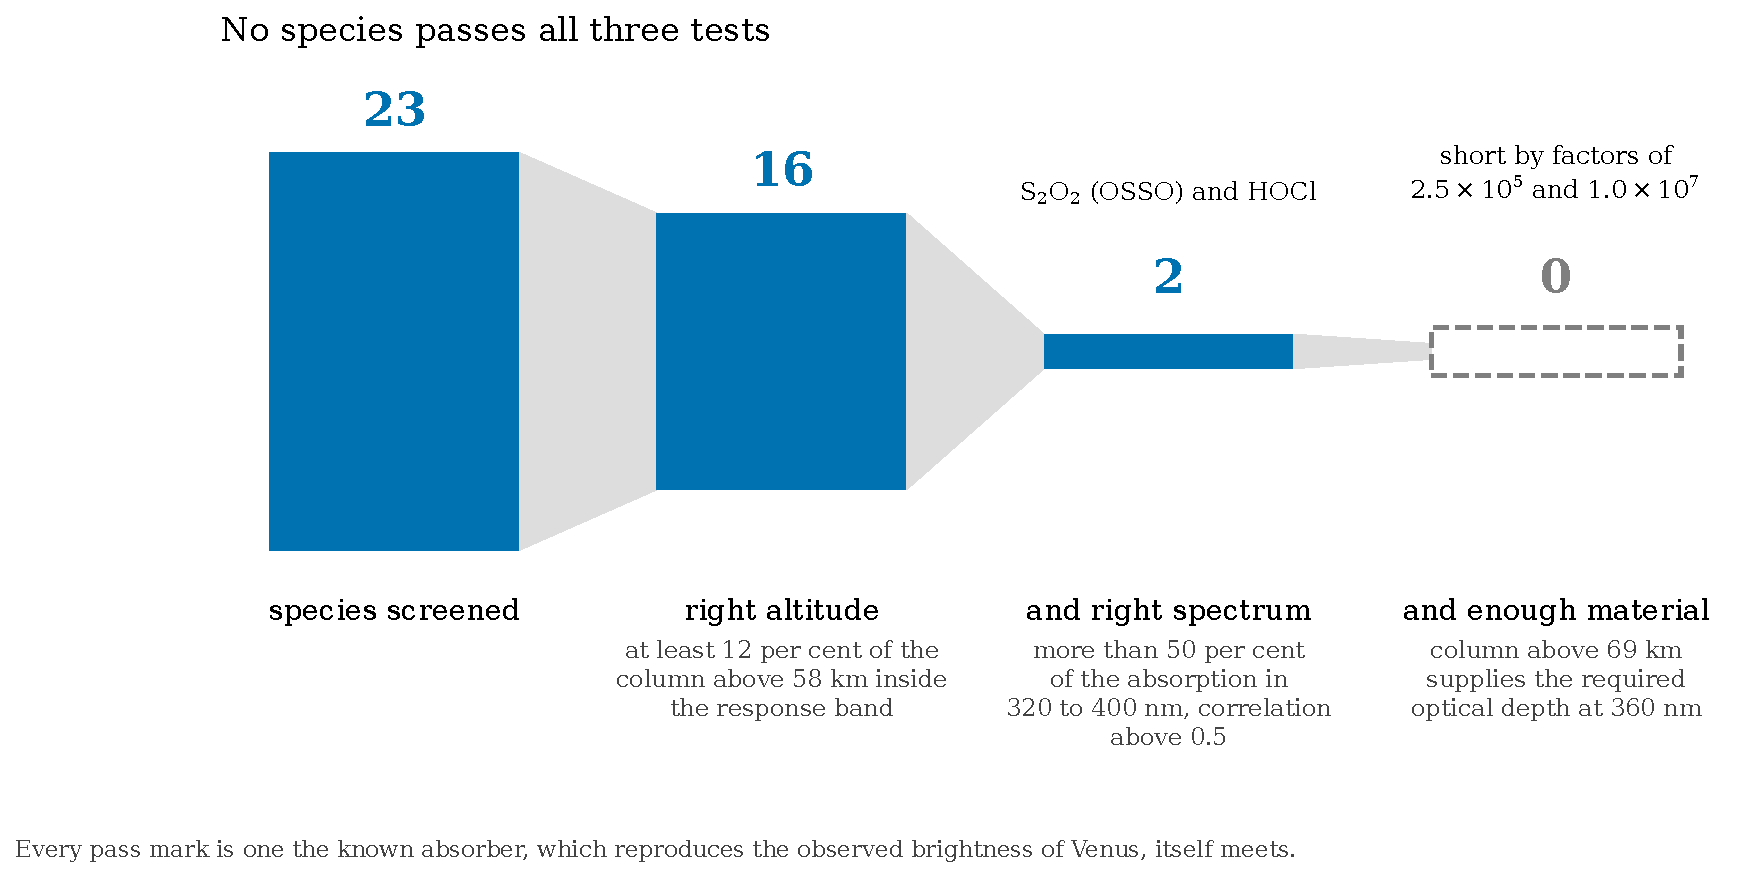
\includegraphics[width=0.92\textwidth]{F03_CTX_three-gates_ch1_backup.pdf}
  \caption[No species passes all three tests (Experiment~12)]{No species passes all three tests (Experiment~12). The 23 species the model
    can test pass through the three tests in turn; each pass mark is one the empirical
    absorber itself meets. The altitude test asks for at least the empirical absorber's
    own share of its column above 58~km inside the response band. Sources: the registry
    keys that begin \texttt{e12.gate}, which hold the counts and the pass marks, and
    \texttt{e12.S2O2.short.360} and \texttt{e12.HOCl.short.360}, which hold the two
    shortfalls. Chapter~8 explains how to read a registry key.}
  \label{fig:F3}
\end{figure}

\section{Objective and Research Gap}
\label{sec:objective}

The objective of Phase 1 was to test, inside a photochemistry and transport model, whether
the proposed carriers of the unknown absorber can meet all three requirements at once,
and to find out which of the three requirements decides the outcome. It was reached
through five steps, each of which became a group of experiments.

\textbf{Make the absorber switchable.} The model had to be able to run with the absorber
on and with it off, differing in nothing else, so that any change could be blamed on the
absorber alone (Chapter~3).

\textbf{Find where the absorber acts.} The response had to be located in amount,
wavelength, chemical reactions and altitude (Experiments~1 to~6, Chapter~5).

\textbf{Find what decides the size of the response.} Moving the absorber up or down was
compared with changing its spectrum, and the model's chemistry was then allowed to place a
candidate by itself (Experiments~7 to~10, Chapters~5 and~6).

\textbf{Test real candidates.} Published spectra and mineral data were tested against the
three requirements (Experiments~11 to~14, Chapter~6).

\textbf{Verify every number.} Every number in this report is recomputed from
the saved model output and checked automatically (Chapter~8).

\textbf{The research gap.} The studies reviewed for this project test candidates mainly on
spectral grounds, and the photochemical models among them treat the absorber either as a
fixed opacity~\cite{dai2024} or examine one candidate at a time~\cite{dai2025review,
egan2025osso}. None of them, as far as this review found, applies the amount, the altitude
and the spectrum requirements together to every species a model can represent, and none
measures how strongly the radiative effect of the absorber depends on its altitude. Phase~1
fills that gap with the following main results:
\begin{itemize}
  \item Altitude is a first-order control. Moving the absorber's profile up by
    17.8439~km changes the radiation field 7.34 times more than moving it down by
    18.0000~km (Experiment~7).
  \item The model's chemistry, not the modeller, decides where a candidate sits, and
    when it is allowed to decide, the candidate falls out of the response band
    (Experiment~9).
  \item No species the model can represent passes all three tests (Experiment~12), and
    the candidate families fail for different reasons.
  \item A published rejection of ferric chloride rests on an absorbance measured in water.
    Measured in hydrochloric acid, ferric chloride absorbs 4 to 25 times more strongly,
    and if it absorbs so in the droplets it becomes a plausible minor component
    (Experiment~14, done after Phase~1 closed). This does not identify the
    absorber.
\end{itemize}
These are negative results for the candidates tested, and they are reported as such.

\section{Organisation of this report}
\label{sec:organisation}

Chapter~2 reviews the papers this project builds on. Chapter~3 describes the model and
the groundwork that made controlled experiments possible. Chapter~4 states the
conventions used for every number. Chapters~5 and~6 describe the fourteen experiments in
the order they were done. Chapter~7 states what Phase~1 establishes and where its limits
lie. Chapter~8 describes how every number was verified and how a reader can trace any
number back to the code. Chapter~9 proposes Phase~2, and Chapter~10 concludes.
